\chapter{Seven-Segment Controller}

\section{Implementation}

\texttt{sev\_seg.sv} multiplexes four digits over the active-low anodes and
segment outputs. The APB registers \texttt{CTL} (\texttt{0x000}) enable the
display, \texttt{VAL} (\texttt{0x004}) holds the digits and decimal points,
and \texttt{DIM} (\texttt{0x008}) controls brightness. The four digits occupy
the low 16 bits of \texttt{VAL}, with digit~0 in bits~3--0. The archived
standalone synthesis results are listed in Table~\ref{tab:resources}.

\section{Module Testbench}

\texttt{sev\_seg\_tb.sv} uses the APB master to write \texttt{0x1234} to
\texttt{VAL}, \texttt{0xF} to \texttt{DIM}, and \texttt{0x1} to \texttt{CTL}.
It checks the readback of all three registers. Figure~\ref{fig:display-setup}
shows the APB transfers and Figure~\ref{fig:display-scan} shows digit~0.

\evidencefigure{sev-seg-waveform.png}{Seven-segment controller waveform from the final source.}{fig:display-final}{Capture the APB transfers and digit scan from the final RTL simulation.}

\begin{figure}[!htbp]
  \centering
  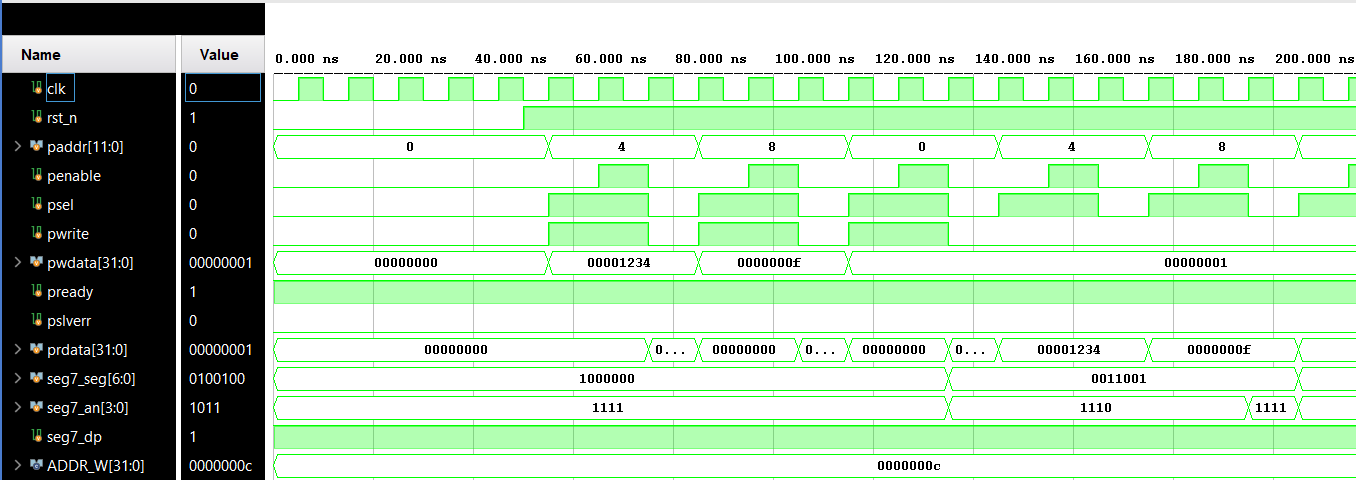
\includegraphics[width=\linewidth]{figures/Lab2/7seg_setup.png}
  \caption{Lab 2 APB writes and readback for the display registers.}
  \label{fig:display-setup}
\end{figure}

\clearpage
\section{Digit Scan}

\begin{figure}[!htb]
  \centering
  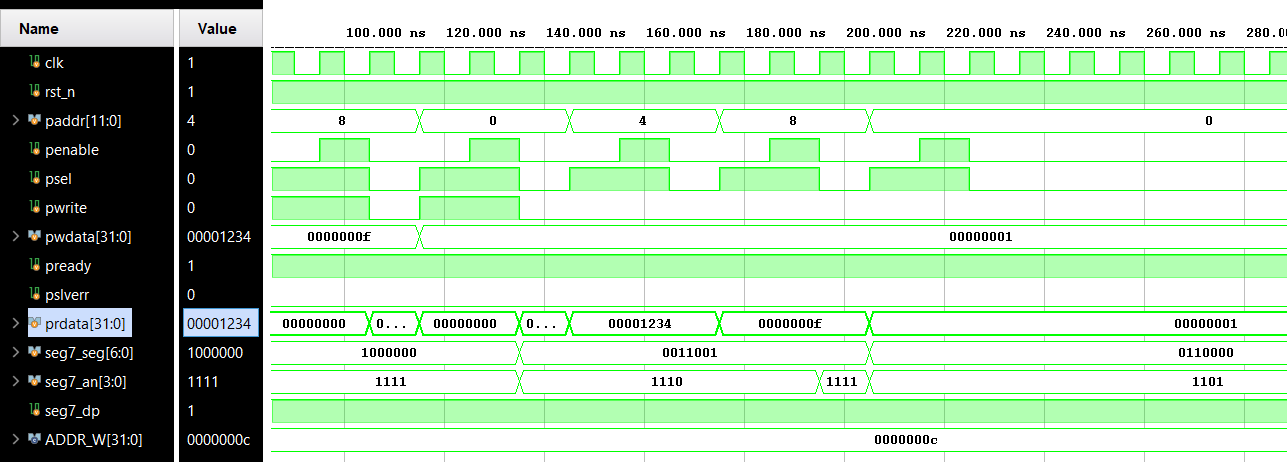
\includegraphics[width=\linewidth]{figures/Lab2/digit0.png}
  \caption{Anode pattern \texttt{1110} selects digit~0, which displays 4.}
  \label{fig:display-scan}
\end{figure}

\section{Lint and Synthesis}

The archived Vivado linter found one \texttt{ASSIGN-10} violation on
\texttt{pwdata}. The first unread bit was bit~17. The register map uses
selected write-data fields for digit values, decimal points, and control.
The archived standalone synthesis log records zero errors and zero critical
warnings. Table~\ref{tab:resources} reports the archived area counts.

\begin{figure}[!htb]
  \centering
  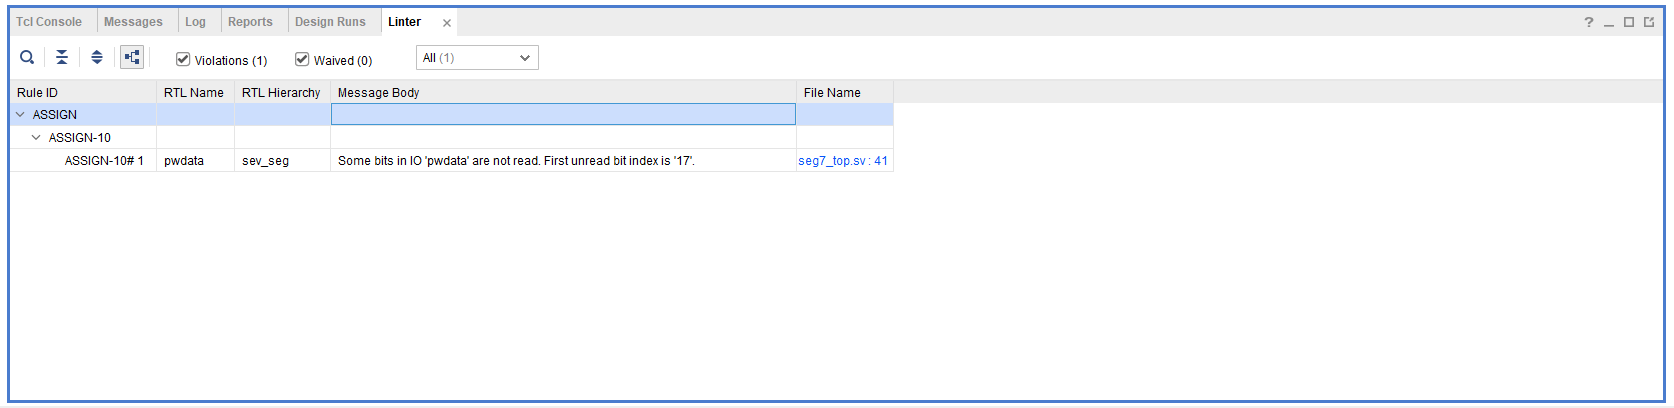
\includegraphics[width=\linewidth,trim=0 172bp 560bp 0,clip]{figures/Lab2/Lab02_sev_seg_linter.png}
  \caption{Vivado lint finding on the seven-segment controller write-data port.}
  \label{fig:sev-seg-lint}
\end{figure}

